\newpage
\chapter{Сериализация объектов}

\section{Концепция и механика сериализации объектов}

\textbf{Сериализация объектов} - это процесс сохранения состояния объектов в виде последовательности байтов. По сути каждый объект (с некоторыми оговорками) можно упаковать в некоторую последовательность файлов, которую затем при помощи потоков и других систем можно передать в другое место с экономией времени и памяти. Для того чтобы можно было управлять данными процессом, используется специальный механизм Java Serialization API.

Для сериализации класса объекта необходимо, чтобы он реализовывал особый интерфейс \verb|java.io.Serializable|. Сам по себе интерфейс не содержит никаких методов для обязательной реализации, он служит маркером для системы, что используемый объект может быть сериализован.

Пример класса, реализующий механизм сериализации:

\begin{lstlisting}
    import java.io.Serializable;
    
    class TestSerial implements Serializable {
      public byte version = 100;
      public byte count = 0;
    }
\end{lstlisting}

Теперь, когда класс может быть сериализован, попробуем записать его в файл \verb|temp.out|:

\begin{lstlisting}
    public static void main(String args[]) throws IOException {
      FileOutputStream fos = new FileOutputStream("temp.out");
      ObjectOutputStream oos = new ObjectOutputStream(fos);
      TestSerial ts = new TestSerial();
      oos.writeObject(ts);
      oos.flush();
      oos.close();
    }
\end{lstlisting}

Ключевым звеном здесь является объект класса \verb|ObjectOutputStream|, который как раз позволяет записать байтовые данные в поток. Для работы над классом можно использовать следующие методы:

\begin{enumerate}
    \item \verb|void close()| — закрытие потока;
    \item \verb|void flush()| — очистка потока и перенос его данных в поток выхода;
    \item \verb|void write(byte[] buf)| — запись массива байтов;
    \item Методы типа \verb|void writeT(T item)|, позволяющие записать значение соответствующего типа, будь-то \verb|int|, \verb|boolean| и пр.;
    \item \verb|void writeObject(Object obj)| — запись самого объекта в поток.
\end{enumerate}

\section{Десериализация}

\textbf{Десериализация} — это обратный сериализации процесс, который позволяет последовательности байтов вновь стать объектом. Для этого в коде Java используется класс \verb|ObjectInputStream|, соответственно извлекающий ранее сериализованные данные из потока.

Возьмём код выше, в котором мы сериализовали объект класса \verb|TestSerial|, и теперь мы десериализуем его:

\begin{lstlisting}
    public static void main(String args[]) throws IOException {
      FileInputStream fis = new FileInputStream("temp.out");
      ObjectInputStream oin = new ObjectInputStream(fis);
      TestSerial ts = (TestSerial) oin.readObject();
      System.out.println("version="+ts.version);
      System.out.println("count="+ts.count);
    }
\end{lstlisting}

При помощи классов \verb|FileInputSteam| и \verb|ObjectInputStream| мы получаем байты информации о классе а затем преобразуем их обратно в объект при помощи метода \verb|readObject()|, возвращающего объект. Приведя его к нужному типу, в консоли вывода мы получим следующую строку:

\begin{lstlisting}
    version=100
    count=0
\end{lstlisting}

Кроме указанного выше метода класс поддерживает также и другие методы:

\begin{enumerate}
    \item \verb|void close()| — закрытие потока;
    \item \verb|int skipBytes(int len)| — пропуск \verb|len| последующих байтов при чтении;
    \item \verb|int available()| — количество оставшихся байтов для чтения;
    \item \verb|int read()| и производные от него — считывает значение одного байта или соответствующего сигнатуре функции объекта.
\end{enumerate}

\section{Классы с запретом на сериализацию и работа с ними}

Несмотря на то, что сериализация предполагает удобный формат передачи данных об объектах класса, иногда она не должна применяться. Так, например, данный процесс не применяется для тех полей, которые:

\begin{enumerate}
    \item вычисляются программно (т.е. на основе другой информации, по ходу выполнения программы);
    \item являются приватными (пароли, уникальные данные и пр.);
    \item не обладают интерфейсом \verb|Serializable| (например, поля классов \verb|Thread|, \verb|OutputStream| и его подклассы, \verb|Socket|;
    \item имеют информацию о состоянии объекта.
\end{enumerate}

Для того чтобы обеспечить отсутствие данных полей с сериализированной последовательности байтов, используется специальное ключевое слово \verb|\textbf{transient}| (технически само поле будет присутствовать, однако его значение всегда будет равно \verb|null|). Так, взяв код определения класса \verb|TestSerial| выше, мы можем запретить сериализацию поля \verb|version|:

\begin{lstlisting}
    import java.io.Serializable;
    
    class TestSerial implements Serializable {
      public transient byte version = 100; // <--
      public byte count = 0;
    }
\end{lstlisting}

Другой способ предполагает полный запрет за сериализацию всего класса вообще — для этого достаточно перегрузить основные методы чтения/записи в поток сериализации:

\begin{lstlisting}
private void writeObject(ObjectOutputStream out) throws IOException

private void readObject(ObjectInputStream in) throws IOException
\end{lstlisting}

При помощи данного кода можно удостовериться, что класс нельзя будет сериализовать подобными функциями — при попытке их вызова выбросится исключение.

\section{Альтернатива сериализации — экстернализация}

Несмотря на то, что сериализация успешно справляется со своими задачами, ей присущи следующие недостатки:

\begin{enumerate}
    \item Низкая производительность за счёт вызова большого количества служебной информации;
    \item Инструментарий ограничения сериализации ограничен лишь запретом отдельных полей через \verb|transient| или класса через перегрузку;
    \item Иногда приходится мучаться со случаями получения "обнулённых" данных — при условии, если пароль и другую конфиденциальную информацию всё же нужно передавать внутренним сервисам.
\end{enumerate}

Для решения данной проблемы имеется альтернатива в виде \textbf{экстернализации} и соответствующего интерфейса \verb|Externalizable|. По сути это та же сериализация, только теперь программист может сам определять правила, по которым данные будут вводиться или выводиться через поток сериализации. В этом случае решаются вышеуказанные проблемы:

\begin{enumerate}
    \item Можно увеличить производительность, вызывая только необходимую информацию;
    \item Инструментарий ограничений сериализации теперь польностью отдан программисту;
    \item Вопрос с паролями и пр. может быть решён за счёт внутренней шифровки чувствительных данных каким-либо алгоритмом шифрования.
\end{enumerate}

Интерфейс \verb|Externalizable| расширяет родительский интерфейс \verb|Serializable| и приводит следующие методы, обязательные к переопределению:

\begin{enumerate}
    \item \verb|void writeExternal(ObjectOutput out)| — запись в поток экстернализации;
    \item \verb|void writeExternal(ObjectInput in)| — чтение из потока экстернализации.
\end{enumerate}

Пример класса, подвергнутого экстернализации, будет выглядеть примерно так:

\begin{lstlisting}
    import java.io.Externalizable;
    import java.io.IOException;
    import java.io.ObjectInput;
    import java.io.ObjectOutput;
    import java.util.Base64;
    
    public class UserInfo implements Externalizable {
    
       private String firstName;
       private String lastName;
       private String password;
    
       private static final long serialVersionUID = 1L;
    
       public UserInfo() {
       }
    
       public UserInfo(String firstName, String lastName, String password) {
           this.firstName = firstName;
           this.lastName = lastName;
           this.password = password;
       }
    
       @Override
       public void writeExternal(ObjectOutput out) throws IOException {
           out.writeObject(this.getFirstName());
           out.writeObject(this.getLastName());
           out.writeObject(this.encryptString(this.getpassword()));
       }
    
       @Override
       public void readExternal(ObjectInput in) throws IOException, ClassNotFoundException {
           firstName = (String) in.readObject();
           lastName = (String) in.readObject();
           password = this.decryptString((String) in.readObject());
       }
    
       private String encryptString(String data) {
           return Base64.getEncoder().encodeToString(data.getBytes());
       }
    
       private String decryptString(String data) {
           return String(Base64.getDecoder().decode(data));
       }
    
       public String getFirstName() {
           return firstName;
       }
    
       public String getLastName() {
           return lastName;
       }
    
       public String getPassword() {
           return password;
       }
    }
\end{lstlisting}

Стоит также отметить, что \textbf{любой класс, имплементирующий интерфейс \texttt{Externalizable}, обязан иметь конструктор по умолчанию} — связано это с особым порядком выполнения десериализации сперва через создание объекта по умолчанию, а затем уже вызова оттуда соответствующих методов.

\chapter{Символьный ввод-вывод}

\section{Символьный ввод-вывод и соответствующие декораторы}

В предыдущих темах мы ознакомились с понятиями библиотек и потоков ввода-вывода, их классами и работой с ними, а также байтовыми классами и декораторами ввода-вывода.

В этой теме речь пойдёт о схожем классе — \textbf{символьном вводе-выводе}. В отличие от байтового, оперирующего только последовательностями байтов и байтовыми потоками, символьный предполагает описание и управление \textbf{символьными последовательностями — строками}. Для этой цели используется отдельный вид потоков — \textbf{символьный поток}.

Символьный поток также разделяется на две категории — поток ввода и вывода, им соответствуют абстрактные классы \verb|Reader| и \verb|Writer| соответственно. Они позволяют создавать и использовать множество дочерних классов, используемых для управления некоторой категории строковых данных.

Для потоков ввода \verb|Reader| является родителем для следующих наиболее распространённых классов-декораторов:

\begin{enumerate}
    \item \verb|FileReader| — позволяет связать символьный файл и поток ввода;
    \item \verb|BufferedReader| — использует буферизованный поток ввода символов (используется для сокращения количества обращений к носителю данных);
    \item \verb|CharArrayReader| — считывает данные из массива символов;
    \item \verb|FilterReader| — использует отфильтрованный некоторым(и) правилом(ами) поток ввода символов.
\end{enumerate}

Также этот родительский абстрактный класс содержит несколько методов, из которых мы выделим основные:

\begin{enumerate}
    \item \verb|int read()| — возвращает представление очередного доступного символа во входном потоке в виде целого числа;
    \item \verb|int read(char[] buffer)| — пытается прочесть максимум \verb|buffer.length| символов из входного потока в массив \verb|buffer|. Возвращает количество символов, в действительности прочитанных из потока;
    \item \verb|int read(char[] buffer, int offset, int length)| - пытается прочесть максимум \verb|length| символов, расположив их в массиве \verb|buffer|, начиная с элемента \verb|offset|. Возвращает количество реально прочитанных символов;
    \item \verb|close()| – метод закрывает поток.
\end{enumerate}

Для потоков вывода \verb|Writer| классы-декораторы в целом схожи, различие лишь в изменении части сигнатуры \verb|Reader| на \verb|Writer|. ЧТо же касается методов, то у \verb|Writer| они отличны от \verb|Reader|:

\begin{enumerate}
    \item \verb|void write(int c)| – записывает один символ в поток;
    \item \verb|void write(char[] buffer)| – записывает массив символов в поток;
    \item \verb|void write(char[] buffer, int offset, int length)| – записывает в поток подмассив символов длиной \verb|length|, начиная с позиции \verb|offset|;
    \item \verb|void write(String aString)| – записывает строку в поток;
    \item \verb|void write(String aString, int offset, int length)| – записывает в поток подстроку символов длиной \verb|length|, начиная с позиции \verb|offset|.
\end{enumerate}

\section{Стандартные потоки ввода-вывода}

Все языки программирования обеспечивают поддержку стандартного ввода/вывода, где программа пользователя может произвести ввод посредством клавиатуры и осуществить вывод на экран компьютера. Если вы знакомы с языками программирования C либо C++, вам должны быть известны три стандартных устройства \verb|STDIN|, \verb|STDOUT| и \verb|STDERR|. Аналогичным образом, Java предоставляет следующие три стандартных потока:

\begin{enumerate}
    \item \textbf{Стандартный ввод} (\verb|STDIN|) – используется для перевода данных в программу пользователя, клавиатура обычно используется в качестве стандартного потока ввода, представленного в виде \verb|System.in|;
    \item \textbf{Стандартный вывод} (\verb|STDOUT|) – производится для вывода данных, полученных в программе пользователя, и обычно экран компьютера используется в качестве стандартного потока вывода, представленного в виде \verb|System.out|;
    \item \textbf{Стандартная ошибка} (\verb|STDERR|) – используется для вывода данных об ошибке, полученной в программе пользователя, чаще всего экран компьютера служит в качестве стандартного потока сообщений об ошибках, представленного в виде \verb|System.err|.
\end{enumerate}

\section{Взаимодействие со стандартными потоками при помощи объектов классов символьного ввода-вывода. Класс Scanner}

Заметим, что с помощью перечисленных ранее классов символьного ввода-вывода можно также передавать данные через консоль ввода-вывода ошибок — причём как прямо на консоль, так и опосредовано, через файлы/фильтры/пр. Рассмотрим следующий пример:

\begin{lstlisting}
import java.io.*;
 
public class Program {
 
    public static void main(String[] args) {
         
        try(BufferedReader br = new BufferedReader (new InputStreamReader(System.in)); 
            BufferedWriter bw = new BufferedWriter(new FileWriter("notes5.txt")))
        {
            String text;
            while(!(text=br.readLine()).equals("ESC")){
                  
                bw.write(text + "\n");
                bw.flush();
            }
        }
        catch(IOException ex){
              
            System.out.println(ex.getMessage());
        } 
    }   
}
\end{lstlisting}

Здесь мы определяем два буферных потока ввода-вывода — \verb|br| и \verb|bw|. Каждый из них при этом использует различный источник: так, поток ввода использует стандартный поток ввода \verb|System.in| вместе с байтовым \verb|InputStreamReader| для получения и передачи байтов информации, полученных через консоль ввода. В свою очередь поток вывода использует файловый поток вывода, связанный с файлом notes5.txt.

Здесь считывается некоторая строка текста, а затем проверяется, не равна ли она строке "ESC" — указателю того, что приём данных должен завершиться. Если строки не равны, то полученная строка сначала передаётся в поток вывода \verb|bw| вместе с \verb|\n| — символом перехода на новую строку — а затем поток очищается, передавая информацию прямо в файл.

Как вы могли заметить, конструкция связи между стандартным а и символьным потоками ввода довольна громоздка, поэтому встаёт вопрос об упрощении получения данных из консоли. Для этого как раз и используется вспомогательный класс \verb|Scanner|, который позволяет напрямую, без помощи байтовых потоков сразу использовать \verb|System.in|. Рассмотрим ещё один пример:

\begin{lstlisting}
import java.util.Scanner;
 
public class Program {
   
    public static void main(String[] args) {
           
        Scanner in = new Scanner(System.in);
        System.out.print("Input name: ");
        String name = in.nextLine();
        System.out.print("Input age: ");
        int age = in.nextInt();
        System.out.print("Input height: ");
        float height = in.nextFloat();
        System.out.printf("Name: %s  Age: %d  Height: %.2f \n", name, age, height);
        in.close();
    }
}
\end{lstlisting}

Здесь мы создаём объект класса \verb|Scanner| под названием \verb|in|, через который мы можем передавать введённые через консоль данные. Сам класс содержит несколько методов, позволяющих это сделать:

\begin{enumerate}
    \item \verb|next()| — считывает введенную строку до первого пробела;
    \item \verb|nextLine()| — считывает всю введенную строку;
    \item \verb|nextInt()| — считывает введенное число целочисленного типа \verb|int|;
    \item \verb|nextDouble()| — считывает введенное число вещественного типа \verb|double|;
    \item \verb|nextBoolean()| — считывает значение булева типа \verb|boolean|;
    \item \verb|nextByte()| — считывает введенное число типа \verb|byte|;
    \item \verb|nextFloat()| — считывает введенное число типа \verb|float|;
    \item \verb|nextShort()| — считывает введенное число \verb|short|;
\end{enumerate}

\chapter{Обработка исключительных ситуаций}

\section{Концепция обработки исключений}

\textbf{Исключительная ситуация} – это программная ошибка, которая возникает во время выполнения последовательности программного кода. Программная ошибка может быть логической ошибкой программиста во время разработки программы. Например, исключительная ситуация может возникать в случаях:

\begin{enumerate}
    \item попытки деления на нуль;
    \item попытки обращения к элементу массива, номер индекса которого выходит за пределы объявленного;
    \item попытки взять корень из отрицательного числа;
    \item попытки открыть файл по имени, которого нет на диске;
    \item другие случаи.
\end{enumerate}

Как правило, каждая исключительная ситуация может иметь свой код ошибки и обработку этого кода (вывод соответствующих сообщений, и т.п.). В языке программирования Java разработан механизм обработки исключительных ситуаций.

В языке программирования Java, \textbf{исключение} – это специальный объект, описывающий исключительную ситуацию, которая возникла в некоторой части программного кода. Объект представляющий исключение, генерируется в момент возникновения исключительной ситуации. После возникновения критической (исключительной) ситуации исключение перехватывается и обрабатывается. Таким образом, возникает понятие \textbf{ генерирования исключения}. Генерирование исключения – процесс создания объекта, который описывает данное исключение.

Исключения могут генерироваться либо автоматически — через исполняемую систему Java, при нарушении ограничений системы языка, — либо вручную — через программный код. Первый случай происходит, если в самом коде нету \textbf{блока обработки и перехвата} исключений или же он имеется, но не обрабатывает данное исключение.

Обычно для блока исключений используются следующие ключевые слова:

\begin{enumerate}
    \item \verb|try| — указывает начало блока кода, в котором возможно исключение(я);
    \item \verb|catch| — указывает начало блока кода, который запускается при срабатывании определённого типа исключения;
    \item \verb|throw| — используется для ручного срабатывания исключения;
    \item \verb|throws| — используется для того, чтобы показать, что данный метод может генерировать исключение, которое он не обрабатывает;
    \item \verb|finally| — указывает начало блока кода, который обязательно выполнится после \verb|try| невзирая на то, были ли перехвачены исключения или нет.
\end{enumerate}

Обычно для перехвата исключения используется конструкция \verb|try...catch|, иногда туда включают и \verb|...finally|. Например:

\begin{lstlisting}
class DemoExceptions {
    double DivNumbers3(int a, int b) {
        double res;
        try {
            res = a/b;
        }
        catch (ArithmeticException e) {
            System.out.println("Division by 0!");
        }
        finally {
            res = 0;
        }
        return res;
    }
}

public class Main {
    public static void main(String[] args) {
        DemoExceptions d = new DemoExceptions();
        double res;
        res = d.DivNumbers3(2, 0);
        System.out.println("res = " + res);
        // Dvision by 0!
        // res = 0.0
    }
}
\end{lstlisting}

\section{Класс Throwable. Виды исключений, иерархия классов исключений}

Базовым классом для всех исключений является класс \verb|Throwable|. От него уже наследуются два класса: \verb|Error| и \verb|Exception|. Все остальные классы являются производными от этих двух классов.

Класс \verb|Error| описывает внутренние ошибки в исполняющей среде Java. Программист имеет очень ограниченные возможности для обработки подобных ошибок.

Собственно исключения наследуются от класса \verb|Exception|. Среди этих исключений следует выделить класс \verb|RuntimeException|. \verb|RuntimeException| является базовым классом для так называемой группы \textbf{непроверяемых исключений} (unchecked exceptions) - компилятор не проверяет факт обработки таких исключений и их можно не указывать вместе с оператором \verb|throws| в объявлении метода. Такие исключения являются следствием ошибок разработчика, например, неверное преобразование типов или выход за пределы массива.

Некоторые из классов непроверяемых исключений:
\begin{enumerate}
    \item \verb|ArithmeticException|: исключение, возникающее при делении на ноль
    \item \verb|IndexOutOfBoundException|: индекс вне границ массива;
    \item \verb|IllegalArgumentException|: использование неверного аргумента при вызове метода
    \item \verb|NullPointerException|: использование пустой ссылки
    \item \verb|NumberFormatException|: ошибка преобразования строки в число
\end{enumerate}

Все остальные классы, образованные от класса \verb|Exception|, называются проверяемыми исключениями (checked exceptions).

Подобные исключения обрабатываются с помощью конструкции \verb|try..catch| Либо можно передать обработку методу, который будет вызывать данный метод, указав исключения после оператора \verb|throws|:

В итоге получается следующая иерархия исключений:

\begin{figure}[h]
\centering
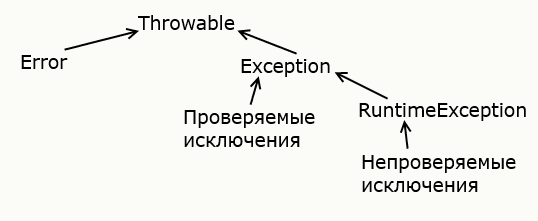
\includegraphics[width=0.8\linewidth]{pic23-1.png}
\label{fig:mpr}
\end{figure}

\section{Пользовательские классы исключений}

Иногда требуется создать свои собственные классы исключений со своей логикой. Для создания своего класса исключений надо унаследовать его от класса \verb|Exception|:

\begin{lstlisting}
class MyExceptionClass extends Exception
{

}
\end{lstlisting}

Данный класс теперь можно использовать в качестве класса исключения в необходимых случаях; кроме того, он может использовать все наследуемые методы класса \verb|Throwable| (например, \verb|getMessage()|, возвращающий описание исключения):

\begin{lstlisting}
public class TrainException {
  public static void main(String[] args) {
    MyExceptionClass mc = new MyExceptionClass();
    String str = mc.getMessage();
    System.out.println("str = " + str);
    // str = null
  }
}
\end{lstlisting}

При этом листинге выведется \verb|str = null|, т.к. сам по себе класс не возвращает сообщения, генерируемого при перехвате объекта исключения.

\section{Генерация исключений}

Как уже упоминалось ранее, ключевое слово \verb|throw| искользуется для принудительной генерации исключений в случае необходимости. Покажем пример:

\begin{lstlisting}
    ...
try {
    // ...
    throw new ThrowableClass(parameters);
}
catch (ThrowableClass e) {
    // ...
}
...
\end{lstlisting}

Внутри блока кода \verb|try| мы вызываем ключевое слово \verb|throw|, а вместе с ним также и объект класса \verb|ThrowableClass| с параметрами (если таковые есть). При этом код внутри изначального блока автоматически прерывается, и происходит переход в блок \verb|catch|, поскольку тип блока соответствует типу выброшенного исключения.

\chapter{Проектирование по контракту, логирование}

\section{Концепция проектирования по контракту, понятия предусловия, постусловия и инварианта класса}

\textbf{Проектирование (программирование) по контракту} –  метод проектирования программного обеспечения, предполагающий документирование (и согласование) прав и обязанностей программных модулей в целях обеспечения корректности программы. Сама программа считается \textbf{корректной}, если она выполняет именно то, что изначально требуется от неё.

Основная идея контрактного программирования — это модель взаимодействия элементов программной системы, основывающаяся на идее взаимных обязательств и преимуществ. Как и в бизнесе, клиент и поставщик действуют в соответствии с определённым контрактом. Контракт некоторого метода или функции может включать в себя:

\begin{enumerate}
    \item конкретные обязательства, которые любой клиентский модуль должен выполнить перед вызовом метода — \textbf{предусловия}, которые дают преимущество для поставщика — он может не проверять выполнение предусловий;
    \item конкретные свойства, которые должны присутствовать после выполнения метода — \textbf{постусловия}, которые входят в обязательства поставщика;
    \item обязательства по выполнению конкретных свойств — \textbf{инвариантов}, которые должны выполняться при получении поставщиком сообщения, а также при выходе из метода.
\end{enumerate}

В целом для контрактного программирования можно выразить следующую идею: «Если клиент, вызывающий подпрограмму, выполняет все предусловия, то вызываемая подпрограмма обязуется, что после ее выполнения все постусловия и инварианты будут истинными». Другими словами, между клиентом и программой заключается некий "контракт", согласно которому обе стороны обязуются выполнять свою часть сделки. Если же одна из сторон так или иначе нарушает свою договорённость, то обычно выполняется специально оговорённая мера: исключение, вывод предупреждения или завершение программы.

Приведём пример кода на Java, основанного на контрактной идее:

\begin{lstlisting}
import com.google.java.contract.*;
import com.google.common.collect.*;
import org.apache.commons.lang3.builder.EqualsBuilder;
import org.apache.commons.lang3.builder.HashCodeBuilder;
 
@Invariant({"title != null && title.length() > 0", "price > 0"})
public class Book {
    private final String title;
    private int price;
 
    @Requires({"title != null && title.length() > 0", "price > 0"})
    public Book(String title, int price) {
        this.title = title;
        this.price = price;
    }
 
    public int getPrice() {
        return price;
    }
 
    @Requires("price > 0")
    public void setPrice(int price) {
        this.price = price;
    }
 
    public String getTitle() {
        return title;
    }
 
    @Override
    public boolean equals(Object obj) {
        return EqualsBuilder.reflectionEquals(this, obj, "price");
    }
 
    @Override
    public int hashCode() {
        return HashCodeBuilder.reflectionHashCode(this, "price");
    }
}

@Invariant("books != null")
public class ShoppingCart {
    private final Multiset<Book> books = HashMultiset.create();
 
    @Requires("book != null")
    @Ensures("books.count(book) == old(books.count(book)) + copies")
    public void addBooks(Book book, int copies) {
        books.add(book, copies);
    }
 
    @Requires({"book != null", "books.count(book) >= copies"})
    @Ensures("books.count(book) == old(books.count(book)) - copies")
    public void removeBooks(Book book, int copies) {
        books.remove(book, copies);
    }
 
    @Requires("book != null")
    @Ensures("books.count(book) == old(books.count(book)) - copies")
    @ThrowEnsures("books.count(book) == old(books.count(book))")
    public void removeBooksUnsafe(Book book, int copies) {
        if (books.count(book) >= copies) {
            books.remove(book, copies);
        } else {
            throw new IllegalStateException("Not enough books to remove");
        }
    }
 
    @Ensures("result >= 0")
    public int getTotal() {
        int total = 0;
        for (Book book : books) {
            total += book.getPrice() * books.count(book);
        }
        return total;
    }
 
    public static void main(String[] args) {
        Book hp = new Book("Harry Potter and the Goblet of Fire", 10);
        Book hhg = new Book("The Hitchhiker's Guide to the Galaxy", 12);
        Book lotr = new Book("The Two Towers", 15);
 
        ShoppingCart cart = new ShoppingCart();
        cart.addBooks(hp, 1);
        cart.addBooks(hhg, 2);
        cart.addBooks(lotr, 3);
        System.out.println("initial total = " + cart.getTotal());
 
        cart.removeBooks(hp, 1);
        System.out.println("total after removing = " + cart.getTotal());
 
        try {
            cart.removeBooksUnsafe(hhg, 4);
        } catch (IllegalStateException e) {
            System.out.println("error message: " + e.getMessage());
        }
        System.out.println("total after exception = " + cart.getTotal());
 
        cart.removeBooks(hhg, 4);
    }
}
\end{lstlisting}

Отметим, что в Java присутствуют специальные аннотации, позволяющие контролировать те или иные концепии контрактов:

\begin{enumerate}
    \item \verb|@Invariant| — проверяет инварианты после выполнения конструктора и всех методов класса — благодаря чему можно контролировать, что основные требуемые функции выполняются;
    \item \verb|@Requires| — проверяет предусловия — выполнение методов допускается в том случае, если передаваемые в него методы соответствуют некоторому условию;
    \item \verb|@Ensures| — проверяет постусловия — позволяет убедиться, что метод действительно выполнил свою часть; работы;
    \item \verb|@ThrowEnsures| — усиленный предыдущий вариант выбрасывающий исключение при нарушении условия.
\end{enumerate}

При создании каждого объекта класса (\verb|Book| и \verb|ShoppingMart|) начинают работать инварианты, позволяющие контролировать свойства и методы — вдруг в результате выполнение критические части будут сломаны или потеряны. Когда выполняется каждый из методов, сначала предъявляются требования к передаваемым переменным от клиента, после чего программный метод выполняет свою работу. При её завершении проверяется, что код действительно выполнил свою часть контракта, а не исказил или проигнорировал данные.

Таким образом, при выполнении контракта можно удостовериться в том, что клиент передаст корректные данные программе, а та корректно обработает их в соответствии с правилами или вернёт ошибку при любых ошибках или несоответствиях.

\section{Логирование и его реализация}

\textbf{Логирование Java} — это процесс, при котором программа на Java-языке записывает сведения о своем исполнении в некий файл или базу данных. Логирование дает возможность отслеживать ход исполнения программы и конкретно кода.

В программировании \textbf{лог} — это специальный файл, который выполняет функцию «бортового журнала» программы. Именно в этот файл, а точнее, в лог программа производит записи о своей работе. Лог-файлы программа может создавать самостоятельно, чтобы вносить туда текстовые пометки.

Лог-файлы помогают «следить» за действиями программы, например, что она функционирует в конкретный момент времени или как она реагирует на действия пользователя.

У одного программного продукта лог-файлы могут быть разные. Например, может быть лог-файл типа:

\begin{enumerate}
    \item \verb|access_log|, в котором фиксируются действия программы при ее взаимодействии с пользователями;
    \item \verb|error_log|, в котором фиксируются все ошибки, произошедшие в результате работы программы;
    \item и пр.
\end{enumerate}

В одном лог-файле может быть множество записей, где каждая строчка будет содержать отдельные результаты для каждого взаимодействия с программой. То есть в каждой записи будет информация о том, что происходило с программным продуктом в конкретный момент времени.

Отметим различия между «логированием» и «логом»:

\begin{enumerate}
    \item Логирование — это процесс, при котором программа прописывает какие-то записи в лог-файлы;
    \item Лог — это сам файл или то место, куда программа производит необходимые записи.
\end{enumerate}

Иногда требуется ограничивать логи по какому-либо критерию: например, они должны содержать только ошибки, либо  только предупреждения, либо содержать все данные. Причиной считается возможное слишком быстрое заполнение лога, из-за становится трудным найти необходимую запись. Поэтому, чтобы контролировать объемы записываемой информации, придумали различные уровни логирования.

Уровни логирования применяются в программах на различных языках программирования, в том числе и на Java. Различают несколько основных уровней, в порядке увеличения данных:

\begin{enumerate}
    \item \verb|OFF| — сообщения не выводятся;
    \item \verb|FATAL| — выводятся фатальные ошибки;
    \item \verb|ERROR| — выводятся обычные ошибки;
    \item \verb|WARNING| — выводятся предупреждения, обычно не приводящие к прерыванию программы;
    \item \verb|INFO| — выводятся обычные и стандартные сообщения;
    \item \verb|DEBUG| — выводится информация, которая пригодится для отладки программы;
    \item \verb|TRACE| — выводится информация для точной отладки;
    \item \verb|ALL| — выводится вся информация.
\end{enumerate}

В таком случае можно внутри программы разграничить логирование таким образом, чтобы сразу видеть, например, основную информацию (в том числе предупреждения и ошибки), либо информацию для дебага, либо всю доступную информацию, либо вообще ничего (впрочем, данный пункт не рекомендуется использовать, если только логирование не влияет на производительность ПК).

Для логирования данных на Java существует несколько специализированных библиотек:

\begin{enumerate}
    \item \verb|java.util.logging (JUL)| (примечателен тем, что поставляется вместе с JDK);
    \item \verb|Apache log4j|;
    \item \verb|logback|;
    \item \verb|Apache log4j2|;
    \item \verb|JCL|;
    \item \verb|SLF4J|;
\end{enumerate}

В основе этих библиотек лежат три понятия:

\begin{enumerate}
    \item \verb|logger| — объект, область ответственности которого - вывод данных в лог и управление уровнем (детализацией) этого вывода;
    \item \verb|appender| — некоторая точка, в которую помещаются все логи и сообщения (файл, БД, консоль и т.п.);
    \item \verb|layout| — как именно данные представляются пользователю.
\end{enumerate}

На данный момент рекомендуется использовать библиотеки \verb|SLF4J| и \verb|logback|, особенно вместе, поскольку они позволяют наиболее полно использовать возможности логирования данных. Тем не менее, в данном учебнике будет рассматривать наиболее простая из представленных выше библиотек — \verb|JUL|.

\section{Библиотека логирования java.util.logging (JUL)}

Эта библиотека-логер, как уже упоминалось ранее, поставляется вместе с JDK. \verb|Layout| данного логера содержит \textbf{дата-время (автоматически), уровень события и, собственно, само сообщение}.

Отдельно поговорим об уровнях событий. В основном они повторяют основные уровни, о которых говорилось ранее, однако имеются отдельные различия в наименованиях: так, все ошибки, фатальные или нет, определяются как \verb|SEVERE|, а отладочные сообщения определяются как \verb|FINE|, \verb|FINER| и \verb|FINEST|, в порядке увеличения вывода дополнительных данных. Так или иначе, грань между близкими друг к другу уровнями довольно тонка, и поэтому, если это возможно, ею можно пренебречь.

Все выводимые данные можно настроить, т.е. указать, куда записывать логи, что именно писать, как писать и т.д. (другими словами, мы можем настроить и \verb|logger|, и \verb|appender|, и \verb|layout|). Для этого используется файл \verb|logging.properties|, куда и записывуются правила для логирования данных. Обычно используют \verb|java.util.logging.ConsoleHandler| и \verb|java.util.logging.FileHandler| для консоли и файлов соответственно; также для них можно настроить \verb|.level| — максимальный уровень данных для вывода; \verb|.limit| — лимит данных и т.п.

Пример кода, использующий данную библиотеку:

\begin{lstlisting}
import java.io.IOException;
import java.nio.file.Files;
import java.nio.file.Paths;
import java.util.logging.Level;
import java.util.logging.Logger;
 
public class JulExample {
 
    public static final Logger logger = Logger.getLogger(
            JulExample.class.getName());
    
    public static void main(String[] args) {
        logger.info("Application started and constructed.");
        logger.warning("Something to warn");
        logger.severe("Something failed.");
        try {
            Files.readAllBytes(Paths.get("/file/does/not/exist"));
        } catch (IOException ioex) {
            logger.log(Level.SEVERE, "Error message", ioex);
        }
    }
 
}
\end{lstlisting}

В результате в консоль выведется следующая информация:

\begin{lstlisting}
Apr 20, 2023 6:00:41 PM JulExample main
INFO: Application started and constructed.
Apr 20, 2023 6:00:41 PM JulExample main
WARNING: Something to warn
Apr 20, 2023 6:00:41 PM JulExample main
SEVERE: Something failed.
java.nio.file.NoSuchFileException: \file\does\not\exist
	at sun.nio.fs.WindowsException.translateToIOException(WindowsException.java:79)
	at sun.nio.fs.WindowsException.rethrowAsIOException(WindowsException.java:97)
	at sun.nio.fs.WindowsException.rethrowAsIOException(WindowsException.java:102)
	at sun.nio.fs.WindowsFileSystemProvider.newByteChannel(WindowsFileSystemProvider.java:230)
	at java.nio.file.Files.newByteChannel(Files.java:361)
	at java.nio.file.Files.newByteChannel(Files.java:407)
	at java.nio.file.Files.readAllBytes(Files.java:3152)
	at JulExample.main(JulExample.java:17)
\end{lstlisting}

\label{pages_total}
